% -------------------------------------------------------------------------
%  MusicFormats Library
%  Copyright (C) Jacques Menu 2016-2023

%  This Source Code Form is subject to the terms of the Mozilla Public
%  License, v. 2.0. If a copy of the MPL was not distributed with this
%  file, you can obtain one at http://mozilla.org/MPL/2.0/.

%  https://github.com/jacques-menu/musicformats
% -------------------------------------------------------------------------

% !TEX root = MusicFormatsUserGuide.tex

% -------------------------------------------------------------------------
\chapter{Raw {\tt xml2ly} usage}
% -------------------------------------------------------------------------

In computer science, the simplest example one can write with a language is often named 'Hello World'. \mf\ abides to this rule, suppling \gitmxmlfile{basic/HelloWorld.xml}:
\begin{lstlisting}[language=MusicXML]
jacquesmenu@macmini: ~/musicformats-git-dev/musicxmlfiles > cat basic/HelloWorld.xml
<?xml version="1.0" encoding="UTF-8" standalone="no"?>
<!DOCTYPE score-partwise PUBLIC
    "-//Recordare//DTD MusicXML 3.0 Partwise//EN"
    "http://www.musicxml.org/dtds/partwise.dtd">
<score-partwise version="3.0">
  <work>
    <work-title>Hello World!</work-title>
    </work>
  <!-- A very minimal MusicXML example -->
  <part-std::list>
    <score-part id="P1">
      <part-name>Music</part-name>
    </score-part>
  </part-std::list>
  <part id="P1">
<!--=========================================================-->
    <measure number="1">
  <!-- A very minimal MusicXML example, part P1, measure 1 -->
      <attributes>
        <divisions>1</divisions>
        <key>
          <fifths>0</fifths>
        </key>
        <time>
          <beats>4</beats>
          <beat-type>4</beat-type>
        </time>
        <clef>
          <sign>G</sign>
          <line>2</line>
        </clef>
      </attributes>
  <!-- A very minimal MusicXML example, part P1, measure 1, before first note -->
      <note>
        <pitch>
          <step>C</step>
          <octave>4</octave>
        </pitch>
        <duration>4</duration>
        <type>whole</type>
      </note>
    </measure>
<!--=========================================================-->
  </part>
</score-partwise>
\end{lstlisting}


% -------------------------------------------------------------------------
\chapter{Redirecting the output and error messages to files}
% -------------------------------------------------------------------------

By default, \standardInput\ and \standardOutput\ are directed to the terminal in which the \xmlToLy\ command has been submitted.

Let's consider the case of \gitmxmlfile{basic/UnknownMaintainerIdentification.xml}:
\begin{lstlisting}[language=Lilypond]
jacquesmenu@macmini: ~/musicformats-git-dev/musicxmlfiles > xml2ly basic/UnknownMaintainerIdentification.xml
*** MusicXML warning *** basic/UnknownMaintainerIdentification.xml:11: creator type "maintainer" is unknown
\version "2.24.0"

% Pick your choice from the next two lines as needed
%myBreak = { \break }
myBreak = {}

% Pick your choice from the next two lines as needed
%myPageBreak = { \pageBreak }
myPageBreak = {}

\header {
    title                = "Hello World!"
    workCreditTypeTitle            = "Hello World!"
    title                = "Hello World!"
}

\paper {
}

\layout {
    \context {
      \Score
      autoBeaming = ##f % to display tuplets brackets
    }
    \context {
      \Voice
    }
}

Part_POne_Staff_One_Voice_One = \absolute {
    \language "nederlands"
    \key c \major
    \numericTimeSignature \time 4/4

    \clef "treble"
    c'1 | % 2
    \barNumberCheck #2
    | % 2
    \barNumberCheck #2
}

\book {
    \score {
        <<

            \new Staff = "Part_POne_Staff_One"
            \with {
            }
            <<
                \context Voice = "Part_POne_Staff_One_Voice_One" <<
                    \Part_POne_Staff_One_Voice_One
                >>
            >>

        >>

        \layout {
            \context {
              \Score
              autoBeaming = ##f % to display tuplets brackets
            }
            \context {
              \Voice
            }
        }

        \midi {
            \tempo 16 = 360
        }
    }

}
Warning message(s) were issued for input line 11
\end{lstlisting}

The \standardOutput\ and \standardError\ are merged into the terminal window, which may not be satisfactory.
This behaviour can be changed using the shell's redirection operators:
\begin{itemize}
\item \code{>}: redirects \standardOutput\ to a file;
\item \code{2>}: redirects \standardError\ to a file.
\end{itemize}

Thus, after executing:
\begin{lstlisting}[language=Terminal]
jacquesmenu@macmini: ~/musicformats-git-dev/musicxmlfiles > xml2ly basic/UnknownMaintainerIdentification.xml > output.ly 2> error.txt
\end{lstlisting}

\fileName{output.ly} contains the \lily\ code produced, and \fileName{error.txt} contains:
\begin{lstlisting}[language=Terminal]
jacquesmenu@macmini: ~/musicformats-git-dev/musicxmlfiles > cat error.txt
*** MusicXML warning *** basic/UnknownMaintainerIdentification.xml:11: creator type "maintainer" is unknown
Warning message(s) were issued for input line 11
\end{lstlisting}


% -------------------------------------------------------------------------
\chapter{The need for options}
% -------------------------------------------------------------------------

Using \xmlToLy\ as in the previous section is somewhat limited. This command:
\begin{lstlisting}[language=Terminal]
jacquesmenu@macmini: ~/musicformats-git-dev/musicxmlfiles > xml2ly basic/MinimalScore.xml > MinimalScore.ly
\end{lstlisting}

leads to this score:\\
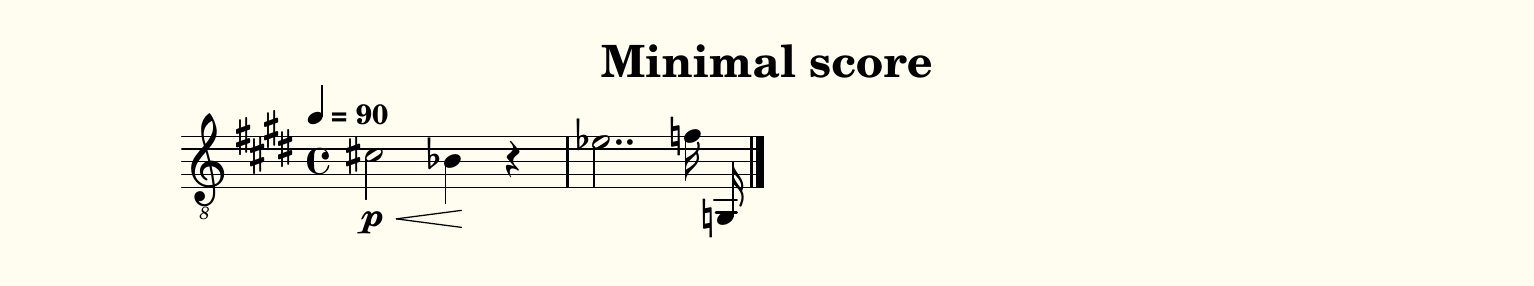
\includegraphics[scale=0.7]{../graphics/MinimalScoreAtDefaultSize.png}

What if we want the \lily\ output to be resized? This is where option come into play. One useful option is:
\begin{lstlisting}[language=Terminal]
jacquesmenu@macmini > xml2ly -query global-staff-size
--- Help for atom "global-staff-size" in subgroup "Layout"
    -global-staff-size, -gss FLOAT
          Set the LilyPond '#(set-global-staff-size ...)' to FLOAT in the LilyPond code.
          FLOAT should be a floating point or integer number.
          The default used by LilyPond is '20.000000'.
\end{lstlisting}

Then:
\begin{lstlisting}[language=Terminal]
jacquesmenu@macmini: ~/musicformats-git-dev/musicxmlfiles > xml2ly basic/MinimalScore.xml -global-staff-size 40 > MinimalScore.ly
\end{lstlisting}

produces that score:\\
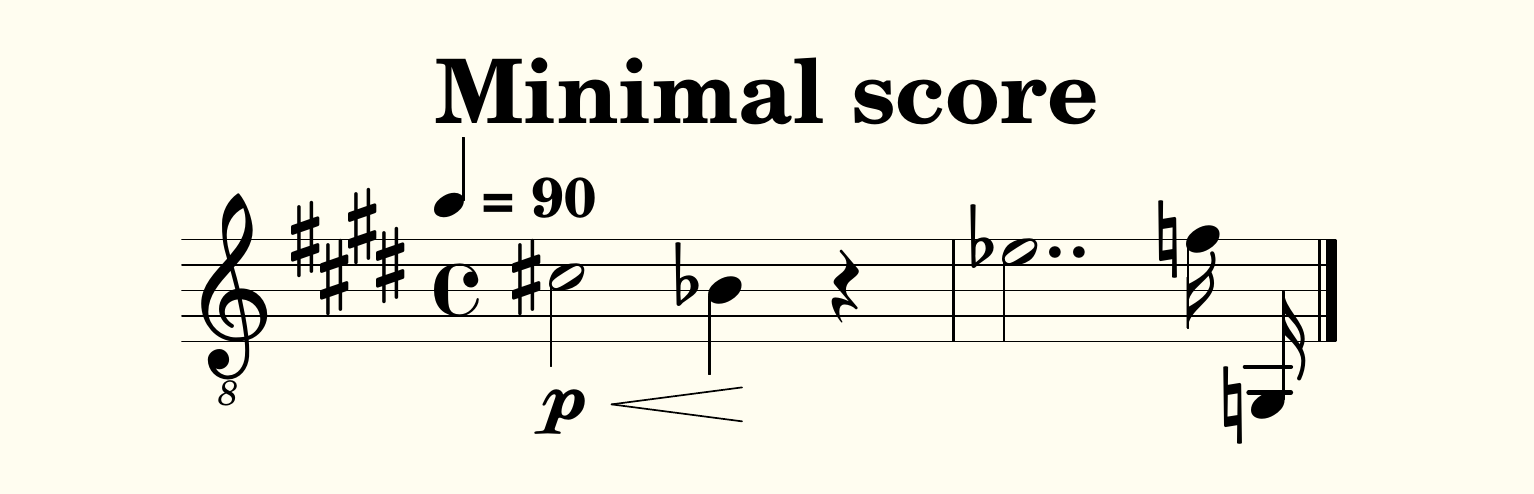
\includegraphics[scale=0.7]{../graphics/MinimalScoreEnlarged.png}

The effect of the \optionNameBoth{global-staff-size}{gss} option is for \xmlToLy\ to generate this at the beginning of the \lily\ output:
\begin{lstlisting}[language=Lilypond]
\version "2.24.0"

% Comment or adapt next line as needed (default is 20)
#(set-global-staff-size 40)

% Pick your choice from the next two lines as needed
%myBreak = { \break }
myBreak = {}

% ... ... ...
\end{lstlisting}

We could of course add this \code{set-global-staff-size} setting by hand, but all \mf\ is about is to automate such things as much as possible. And this is why there are so many options, which in turn explains why the \oahRepr\ infrastructure has been created.

